\documentclass{beamer}
\usetheme{Antibes}
\usepackage{xcolor, colortbl}
\usepackage{algorithm}
\usepackage[noend]{algpseudocode}
\usepackage{textcomp}
\usepackage{listings}
\usepackage{hyperref}
\usepackage{alltt}
\usepackage{tikz}
\usepackage{framed}
\usepackage{marvosym}
\usepackage{wasysym}
\usepackage{marvosym}
\usepackage{crayola}
\usepackage{mathpartir}
\usepackage{tabularx}
\usepackage[belowskip=-15pt,aboveskip=0pt]{caption}
\usepackage[skins]{tcolorbox}
\usepackage{multicol}
\usetikzlibrary{positioning,shapes,arrows, backgrounds, fit, shadows, automata}
\usetikzlibrary{decorations.markings}
%\usepackage{wasysym}
%\usepackage{marvosym}
\setbeamertemplate{footline}[frame number]
%\usecolortheme{fly}
\usefonttheme{serif}

\title[Sujit]{Parsing}
\author{Sujit Kumar Chakrabarti}
\institute{IIITB}
\date{}
\begin{document}
\maketitle

\definecolor{lightblue}{rgb}{0.8,0.93,1.0} % color values Red, Green, Blue
\definecolor{darkblue}{rgb}{0,0,0.5} % color values Red, Green, Blue
\definecolor{Blue}{rgb}{0,0,1.0} % color values Red, Green, Blue
\definecolor{darkgreen}{rgb}{0,0.7,0.2} % color values Red, Green, Blue
\definecolor{Red}{rgb}{1,0,0} % color values Red, Green, Blue
\definecolor{Pink}{rgb}{0.7,0,0.2}
\definecolor{links}{HTML}{2A1B81}
\definecolor{mydarkgreen}{HTML}{126215}
\definecolor{mychoco}{HTML}{5C3317}

\newcommand{\myheader}[1]{
	{\color{purple}
		\begin{Large}
			\begin{center}
				{#1}
			\end{center}
		\end{Large}
	}
}
\newcommand{\myminorheader}[1]{
	{\color{purple}
		\begin{large}
			{#1}
		\end{large}
	}
}

\newcommand{\myprod}[0]{\hspace{0.5cm}$\rightarrow$\hspace{0.5cm}}
\newcommand{\mychoice}[0]{\hspace{0.75cm}$|$\hspace{0.25cm}}
\newcommand{\myderiv}[0]{\hspace{0.5cm}$\Rightarrow$\hspace{0.5cm}}


\lstdefinestyle{javacode}{
	language = Java,
	basicstyle = \ttfamily\scriptsize,
	stringstyle = \ttfamily,
	keywordstyle=\color{Blue}\bfseries,
	identifierstyle=\color{Pink},
	commentstyle=\color{darkgreen},
	frame=single,
	frameround=tttt,
	mathescape=true,
	showstringspaces=false
}

\lstdefinestyle{camlcode}{
	language = Caml,
	basicstyle = \scriptsize\ttfamily,
	stringstyle = \color{red}\ttfamily,
	keywordstyle=\color{Blue}\bfseries,
	identifierstyle=\ttfamily,
	frame=single,
	frameround=tttt,
	numbers=none,
	showstringspaces=false,
	mathescape=true,
	escapeinside={(*@}{@*)}
}

\lstdefinestyle{outputcode}{
	language = bash,
	backgroundcolor = \color{black},
	basicstyle = \tiny\ttfamily\color{white},
	stringstyle = \color{red}\ttfamily,
	keywordstyle=\color{white}\bfseries,
	identifierstyle=\ttfamily,
	frameround=tttt,
	numbers=none,
	showstringspaces=false,
	mathescape=true,
	escapeinside={(*@}{@*)}
}


\mathchardef\mhyphen="2D

% frame begin %%%%%%%%%%%%%%%%%%%%%%%%
\begin{frame}[fragile]{Parsing}

\begin{itemize}
	\item Process of determining if the input belongs to the language of the grammar	
	\item Builds a \textit{parse tree}
\end{itemize}
\end{frame}
% frame end %%%%%%%%%%%%%%%%%%%%%%%%

% frame begin %%%%%%%%%%%%%%%%%%%%%%%%
\begin{frame}[fragile]{Parsing}
{Example}
\begin{center}
\textbf{12:10:45}
\end{center}

\textbf{Specification}: A number followed by a colon followed by a number followed by a colon followed by a number.

\textbf{Regular expression:} num COLON num COLON num

\end{frame}
% frame end %%%%%%%%%%%%%%%%%%%%%%%%

% frame begin %%%%%%%%%%%%%%%%%%%%%%%%
\begin{frame}[fragile]{Parsing}
{Example}
\begin{quote}
12:10:45 \\
11:09:22 \\
...
\end{quote}

\textbf{Specification}: A sequence of a number followed by a colon followed by a number followed by a colon followed by a number.

\textbf{Regular expression:} (num COLON num COLON num)+

\end{frame}
% frame end %%%%%%%%%%%%%%%%%%%%%%%%


% frame begin %%%%%%%%%%%%%%%%%%%%%%%%
\begin{frame}[fragile]{Parsing}
{Example}
\begin{scriptsize}
\begin{multicols}{2}
\begin{quote}
() \\
(() ()) \\
((())) () \\
\end{quote}

\textbf{\color{BrickRed}Specification}: A language of balanced parentheses

\textbf{\color{BrickRed}Regular expression:} ?
\end{multicols}
\end{scriptsize}

\pause

\begin{tiny}
\textbf{\color{BrickRed}Parsing algorithm:}
\begin{center}
\begin{minipage}{0.6\textwidth}
\begin{algorithmic}[0]
\Procedure{balanced-parentheses}{$buffer$}
	\State $level \gets 0$
	\While{$buffer$ has more characters}
		\State $c \gets$ \Call{nextChar}{$buffer$}
		\If{$c$ = LPAREN}
			\State $level \gets level + 1$
		\ElsIf {$c$ = RPAREN}
			\State $level \gets level - 1$
		\EndIf
		\If{$level < 0$}
			\State \textbf{return} $false$
		\EndIf
	\EndWhile
		\If{$level = 0$}
			\State \textbf{return} $true$
		\Else
			\State \textbf{return} $false$
		\EndIf
\EndProcedure
\end{algorithmic}
\end{minipage}
\end{center}
\end{tiny}

\end{frame}
% frame end %%%%%%%%%%%%%%%%%%%%%%%%

% frame begin %%%%%%%%%%%%%%%%%%%%%%%%
\begin{frame}[fragile]{Parsing}
{Examples of structures that can't be expressed using regular expressions}
\begin{lstlisting}[style=camlcode]
(* ... (* ... (* ... *)*)*)
\end{lstlisting}
\begin{lstlisting}[style=camlcode]
let ... in
let ... in 
let in $e$ 
\end{lstlisting}
\begin{lstlisting}[style=javacode]
if(...) {
  if(...) {
    ...
  }
}
\end{lstlisting}

\end{frame}
% frame end %%%%%%%%%%%%%%%%%%%%%%%%


% frame begin %%%%%%%%%%%%%%%%%%%%%%%%
\begin{frame}[fragile]{Context Free Grammar}
{Example: Balanced parentheses}

\pause
\begin{scriptsize}

\begin{framed}
\begin{tabular}{l @{} c @{} l}
$S$     & {\myprod}   & $\epsilon$         \\
$S$     & {\myprod}   & $(S)$         \\
$S$     & {\myprod}   & $S\ S$             \\
\end{tabular}
\end{framed}
\begin{itemize}
\item {\bf Components of a grammar:} Rules/productions, terminals, non-terminals, start symbol
\item \textbf{Meta-language:} language in which the grammar is written; terminals, non-terminals are grammar-symbols/tokens in the meta-language.
\item {\bf Notational variances:} \texttt{::=} instead of \myprod 
\item Could be rewritten as:

\begin{framed}
\begin{tabular}{l @{} c @{} l}
$S$     & {\myprod}   & $\epsilon$         \\
        & {\mychoice}   & $(S)$         \\
        & {\mychoice}   & $S\ S$             \\
\end{tabular}
\end{framed}
\end{itemize}
\end{scriptsize}
\end{frame}
% frame end %%%%%%%%%%%%%%%%%%%%%%%%

% frame begin %%%%%%%%%%%%%%%%%%%%%%%%
\begin{frame}[fragile]{Parsing}
{Grammar}

\textbf{Example:} Grammar for arithmetic expressions
\vspace*{1cm}
\pause

\begin{framed}
\begin{tabular}{l @{} c @{} l}
$E$     & {\myprod}   & $E$ + $E$         \\
$E$     & {\myprod}   & $E$ * $E$         \\
$E$     & {\myprod}   & ($E$)             \\
$E$     & {\myprod}   & 0 $|$ 1 ... $|$ 9 \\
\end{tabular}
\end{framed}

\end{frame}
% frame end %%%%%%%%%%%%%%%%%%%%%%%%

% frame begin %%%%%%%%%%%%%%%%%%%%%%%%
\begin{frame}[fragile]{Grammar}
{\textbf{Example:} Grammar for function call}
\vspace*{1cm}
\pause

\begin{scriptsize}
\begin{framed}
\begin{tabular}{l @{} c @{} l}
$fcall$  & {\myprod}   & \textbf{id} ( arglist )       \\
$arglist$    & {\myprod}   & $arg *$                       \\
$arg$        & {\myprod}   & $exp$                         \\
$exp$        & {\myprod}   & ... $|$ \textbf{SL} $|$ ...   \\
\end{tabular}
\end{framed}

\textbf{Note:}
\begin{itemize}
\item This grammar contains multiple non-terminals.
\item $arglist$ \myprod\ $arg *$ shorthand for \\
\begin{framed}
\begin{quotation}
$arglist$ \myprod\ $\epsilon$ \\
$arglist$ \myprod\ $arg\ arglist$
\end{quotation}
\end{framed}
\end{itemize}
\end{scriptsize}
\end{frame}
% frame end %%%%%%%%%%%%%%%%%%%%%%%%


% frame begin %%%%%%%%%%%%%%%%%%%%%%%%
\begin{frame}[fragile]{Parsing}
{Derivation -- Verifying $i \in L$}
((())) ()
\pause
\begin{itemize}
	\item $S$
	\item $S\ S$
	\item $(S) (S)$
	\item $((S)) (\epsilon)$
	\item $(((S))) ()$
	\item $(((\epsilon))) ()$
	\item $((())) ()$

\end{itemize}
\end{frame}
% frame end %%%%%%%%%%%%%%%%%%%%%%%%

% frame begin %%%%%%%%%%%%%%%%%%%%%%%%
\begin{frame}[fragile]{Parsing}
{Derivation}

\pause
\textbf{Example:} Derivations for arithmetic expressions
\begin{itemize}
	\item 5
	\item 1 + 2
	\item 1 + 2 * 3
\end{itemize}
\end{frame}
% frame end %%%%%%%%%%%%%%%%%%%%%%%%

% frame begin %%%%%%%%%%%%%%%%%%%%%%%%
\begin{frame}[fragile]{Parsing}
{Parse Tree}
\begin{lstlisting}
printf("Hello World!");
\end{lstlisting}

\pause
\textbf{After lexical analysis:}
\begin{center}
\resizebox{0.8\textwidth}{!}{%
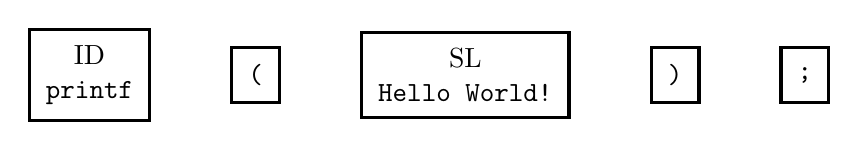
\begin{tikzpicture}[auto,
    ->,
  %  shorten >=2pt,
    >=stealth,
  %  node distance=1cm,
    bb/.style={%
      rectangle, draw=black, very thick, fill=white,
      text ragged, minimum height=2em, inner sep=6pt, align=center
    },
    inv/.style={%
      rectangle, draw=none, fill=white,
      text ragged, minimum height=2em, inner sep=6pt, align=center
    }
]
    \node[bb] (6)                  {ID \\ \texttt{printf}};
    \node[bb] (7)  [right = of 6]  {\texttt{(}};
    \node[bb] (8)  [right = of 7]  {SL \\\texttt{Hello World!}};
    \node[bb] (9)  [right = of 8]  {\texttt{)}};
    \node[bb] (10) [right = of 9]  {\texttt{;}};

  \end{tikzpicture}
}

\end{center}

\end{frame}
% frame end %%%%%%%%%%%%%%%%%%%%%%%%

% frame begin %%%%%%%%%%%%%%%%%%%%%%%%
\begin{frame}{Parsing}
{Parse Tree}

\begin{center}
\resizebox{!}{0.7\textheight}{%
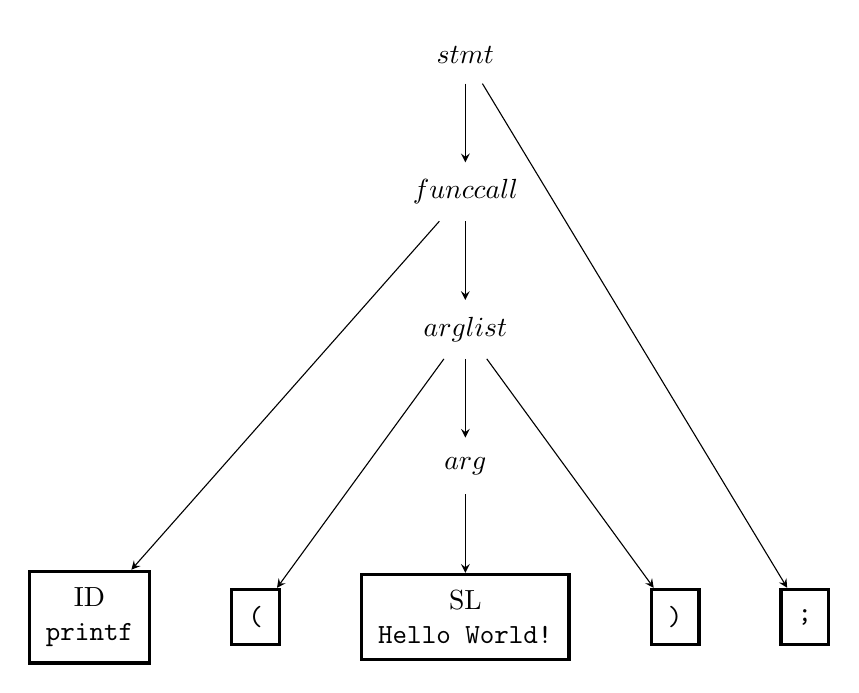
\begin{tikzpicture}[auto,
    ->,
  %  shorten >=2pt,
    >=stealth,
  %  node distance=1cm,
    bb/.style={%
      rectangle, draw=black, very thick, fill=white,
      text ragged, minimum height=2em, inner sep=6pt, align=center
    },
    inv/.style={%
      rectangle, draw=none, fill=white,
      text ragged, minimum height=2em, inner sep=6pt, align=center
    }
]
    \node[bb] (6)                  {ID \\ \texttt{printf}};
    \node[bb] (7)  [right = of 6]  {\texttt{(}};
    \node[bb] (8)  [right = of 7]  {SL \\\texttt{Hello World!}};
    \node[bb] (9)  [right = of 8]  {\texttt{)}};
    \node[bb] (10) [right = of 9]  {\texttt{;}};
    \onslide<2->\node[inv] (11) [above = of 8]  {$arg$};
    \path (11) edge node {}  (8)
    ;
    \onslide<3->\node[inv] (12) [above = of 11]  {$arglist$};
	\path (12) edge node {}  (7)
          (12) edge node {}  (11)
          (12) edge node {}  (9)
    ;
    \onslide<4->\node[inv] (13) [above = of 12]  {$func\mhyphen call$};
    \path (13) edge node {}  (12)
          (13) edge node {}  (6)
    ;

    \onslide<5->\node[inv] (14) [above = of 13]  {$stmt$};
    \path (14) edge node {}  (13)
          (14) edge node {}  (10)
    ;

  \end{tikzpicture}
}

\end{center}

\end{frame}
% frame end %%%%%%%%%%%%%%%%%%%%%%%%


% frame begin %%%%%%%%%%%%%%%%%%%%%%%%
\begin{frame}{Parsing}
{Abstract Syntax Tree}

\begin{center}
\resizebox{!}{0.7\textheight}{%
\begin{tikzpicture}[auto,
    ->,
  %  shorten >=2pt,
    >=stealth,
  %  node distance=1cm,
    bb/.style={%
      rectangle, draw=black, very thick, fill=white,
      text ragged, minimum height=2em, inner sep=6pt, align=center
    },
    inv/.style={%
      rectangle, draw=none, fill=white,
      text ragged, minimum height=2em, inner sep=6pt, align=center
    }
]
    \node[bb] (6)                  {ID \\ \texttt{printf}};
    \node[bb] (7)  [right = of 6]  {\texttt{(}};
    \node[bb] (8)  [right = of 7]  {SL \\\texttt{Hello World!}};
    \node[bb] (9)  [right = of 8]  {\texttt{)}};
    \node[bb] (10) [right = of 9]  {\texttt{;}};
    \node[inv] (11) [above = of 8]  {$arg$};
    \path (11) edge node {}  (8)
    ;
    \node[inv] (12) [above = of 11]  {$arglist$};
	\path 
%	      (12) edge node {}  (7)
          (12) edge node {}  (11)
%          (12) edge node {}  (9)
    ;
    \node[inv] (13) [above = of 12]  {$func\mhyphen call$};
    \path (13) edge node {}  (12)
          (13) edge node {}  (6)
    ;

    \node[inv] (14) [above = of 13]  {$stmt$};
    \path (14) edge node {}  (13)
 %         (14) edge node {}  (10)
    ;

  \end{tikzpicture}
}

\end{center}

\end{frame}
% frame end %%%%%%%%%%%%%%%%%%%%%%%%

% frame begin %%%%%%%%%%%%%%%%%%%%%%%%
\begin{frame}{Parsing}
{Parse Tree}

\begin{itemize}
	\item Grammar symbol $\mapsto$ Nodes
	\item Starting symbol $\mapsto$ Root node
	\item Non-terminals $\mapsto$ internal nodes
	\item Terminals $\mapsto$ leaves
	\item Productions $\mapsto$ Edges
\end{itemize}
\end{frame}
% frame end %%%%%%%%%%%%%%%%%%%%%%%%

% frame begin %%%%%%%%%%%%%%%%%%%%%%%%
\begin{frame}{Parsing}
{Ambiguity}

\begin{center}

\begin{tabular}{c @{\hspace{0.5cm}} c}
1 + 2 * 3
&
\begin{minipage}{0.5\textwidth}
\begin{tcolorbox}
\begin{tabular}{l @{} c @{} l}
$E$     & {\myprod}   & $E$ + $E$         \\
$E$     & {\myprod}   & $E$ * $E$         \\
$E$     & {\myprod}   & ($E$)             \\
$E$     & {\myprod}   & 0 $|$ 1 ... $|$ 9 \\
\end{tabular}
\end{tcolorbox}
\end{minipage}
\end{tabular}
\end{center}

\pause
\begin{center}
\begin{tabular}{c @{\hspace{0.5cm}} c}
\resizebox{!}{0.35\textheight}{%
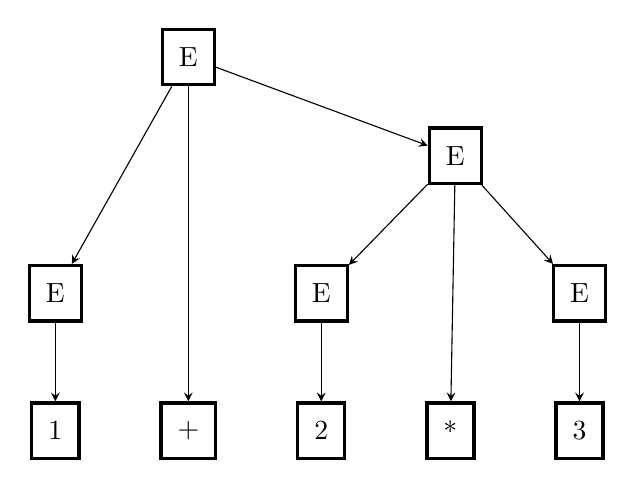
\begin{tikzpicture}[auto,
    ->,
  %  shorten >=2pt,
    >=stealth,
  %  node distance=1cm,
    bb/.style={%
      rectangle, draw=black, very thick, fill=white,
      text ragged, minimum height=2em, inner sep=6pt, align=center
    },
    inv/.style={%
      rectangle, draw=none, fill=white,
      text ragged, minimum height=2em, inner sep=6pt, align=center
    }
]
    \node[bb] (1)                  {1};
    \node[bb] (2)  [right = of 1]  {+};
    \node[bb] (3)  [right = of 2]  {2};
    \node[bb] (4)  [right = of 3]  {*};
    \node[bb] (5)  [right = of 4]  {3};
    \node[bb] (6)  [above = of 1]  {E};
    \node[bb] (7)  [above = of 3]  {E};
    \node[bb] (8)  [above = of 5]  {E};
    \node[bb] (9) [above right = of 7]  {E};
    \node[bb] (10) [above = of 2, yshift = 3cm]  {E};

    \path (6)  edge node {}  (1)
          (10) edge node {}  (2)
		  (10) edge node {}  (6)
		  (10) edge node {}  (9)
		  (9) edge node {}  (8)
		  (9) edge node {}  (4)
		  (9) edge node {}  (7)
		  (7) edge node {}  (3)
		  (8) edge node {}  (5)
    ;

  \end{tikzpicture}
}

\pause
&
\resizebox{!}{0.35\textheight}{%
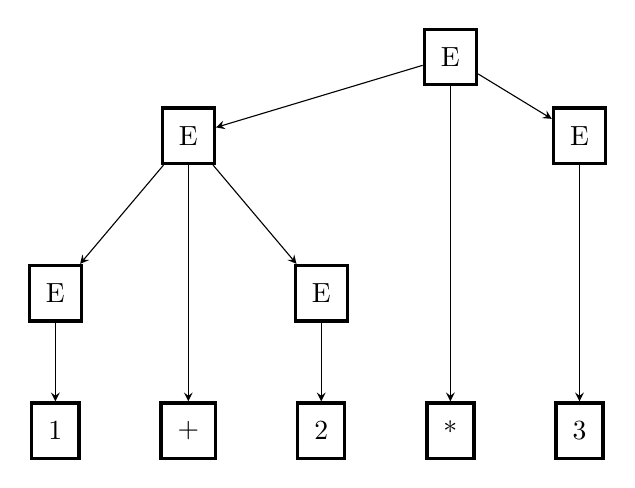
\begin{tikzpicture}[auto,
    ->,
  %  shorten >=2pt,
    >=stealth,
  %  node distance=1cm,
    bb/.style={%
      rectangle, draw=black, very thick, fill=white,
      text ragged, minimum height=2em, inner sep=6pt, align=center
    },
    inv/.style={%
      rectangle, draw=none, fill=white,
      text ragged, minimum height=2em, inner sep=6pt, align=center
    }
]
    \node[bb] (1)                  {1};
    \node[bb] (2)  [right = of 1]  {+};
    \node[bb] (3)  [right = of 2]  {2};
    \node[bb] (4)  [right = of 3]  {*};
    \node[bb] (5)  [right = of 4]  {3};
    \node[bb] (6)  [above = of 1]  {E};
    \node[bb] (7)  [above = of 3]  {E};
    \node[bb] (8)  [above = of 2, yshift = 2cm]  {E};
    \node[bb] (9)  [above = of 5, yshift = 2cm]  {E};
    \node[bb] (10) [above = of 4, yshift = 3cm]  {E};

    \path (6)  edge node {}  (1)
		  (7) edge node {}  (3)
		  (10) edge node {}  (4)
		  (10) edge node {}  (8)
		  (10) edge node {}  (9)
		  (9) edge node {}  (5)
		  (8) edge node {}  (7)
		  (8) edge node {}  (6)
          (8) edge node {}  (2)
    ;

  \end{tikzpicture}
}
\end{tabular}

\end{center}

\end{frame}
% frame end %%%%%%%%%%%%%%%%%%%%%%%%

% frame begin %%%%%%%%%%%%%%%%%%%%%%%%
\begin{frame}{Parsing}
{Ambiguity}

\begin{itemize}
\item Language processors can't deal with ambiguity.
\item Ambiguous grammars are common.
\item Methods of dealing with ambiguity:
\begin{itemize}
	\item Fixing the grammar
	\item Associativity
	\item Operator precedence
\end{itemize}
\end{itemize}
\end{frame}
% frame end %%%%%%%%%%%%%%%%%%%%%%%%

% frame begin %%%%%%%%%%%%%%%%%%%%%%%%
\begin{frame}[fragile]{Parsing}
{Handling Ambiguity -- Fixing the grammar}

\myminorheader{Dangling else}
\begin{center}

\begin{tcolorbox}
\begin{tabular}{l @{} c @{} l}
$stmt$     & {\myprod}     & \textbf{if} $expr$ \textbf{then} $stmt$ \textbf{else} $stmt$  \\
           & {\mychoice}   & \textbf{if} $expr$ \textbf{then} $stmt$                       \\
\end{tabular}
\end{tcolorbox}
\end{center}

\begin{lstlisting}[style=javacode]
if $C_1$ then
  if $C_2$ then
    $S_1$
  else
    $S_2$
\end{lstlisting}

\end{frame}
% frame end %%%%%%%%%%%%%%%%%%%%%%%%

% frame begin %%%%%%%%%%%%%%%%%%%%%%%%
\begin{frame}{Parsing}
{Handling Ambiguity -- Fixing the grammar}

\myminorheader{Dangling else}
\begin{center}

\begin{tcolorbox}
\begin{tabular}{l @{} c @{} l}
$stmt$     & {\myprod}     & \textbf{if} $expr$ \textbf{then} $stmt$ \textbf{else} $stmt$  \\
           & {\mychoice}   & \textbf{if} $expr$ \textbf{then} $stmt$                       \\
\end{tabular}
\end{tcolorbox}

\begin{tcolorbox}
\resizebox{\textwidth}{!}{

\begin{tabular}{l @{} c @{} l}
$stmt$     & {\myprod}     & $matched\_stmt$  \\
           & {\mychoice}   & $open\_stmt$     \\

$matched\_stmt$  & {\myprod}     & \textbf{if} $expr$ \textbf{then} $matched\_stmt$ \textbf{else} $matched\_stmt$  \\
                 & {\mychoice}   & \textbf{other}                                                                  \\
$open\_stmt$     & {\myprod}     & \textbf{if} $expr$ \textbf{then} $stmt$                                         \\
                 & {\mychoice}   & \textbf{if} $expr$ \textbf{then} $matched\_stmt$ \textbf{else} $open\_stmt$     \\
\end{tabular}
}
\end{tcolorbox}
\end{center}
\end{frame}
% frame end %%%%%%%%%%%%%%%%%%%%%%%%


% frame begin %%%%%%%%%%%%%%%%%%%%%%%%
\begin{frame}[fragile]{Parsing}
{Handling Ambiguity -- Operator Precedence}

\begin{scriptsize}

\begin{center}

\begin{tabular}{c @{\hspace{0.5cm}} c}
1 + 2 * 3
&
\begin{minipage}{0.5\textwidth}
\begin{tcolorbox}
\begin{tabular}{l @{} c @{} l}
$E$     & {\myprod}   & $E$ + $E$         \\
$E$     & {\myprod}   & $E$ * $E$         \\
$E$     & {\myprod}   & ($E$)             \\
$E$     & {\myprod}   & 0 $|$ 1 ... $|$ 9 \\
\end{tabular}
\end{tcolorbox}
\end{minipage}
\end{tabular}
\pause

* has higher precedence than +.

\end{center}

\pause
\begin{center}
\begin{tabular}{c @{\hspace{0.5cm}} c}
\resizebox{!}{0.35\textheight}{%
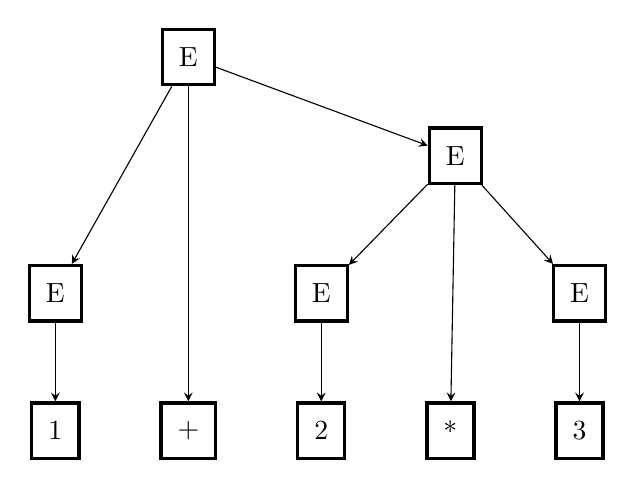
\begin{tikzpicture}[auto,
    ->,
  %  shorten >=2pt,
    >=stealth,
  %  node distance=1cm,
    bb/.style={%
      rectangle, draw=black, very thick, fill=white,
      text ragged, minimum height=2em, inner sep=6pt, align=center
    },
    inv/.style={%
      rectangle, draw=none, fill=white,
      text ragged, minimum height=2em, inner sep=6pt, align=center
    }
]
    \node[bb] (1)                  {1};
    \node[bb] (2)  [right = of 1]  {+};
    \node[bb] (3)  [right = of 2]  {2};
    \node[bb] (4)  [right = of 3]  {*};
    \node[bb] (5)  [right = of 4]  {3};
    \node[bb] (6)  [above = of 1]  {E};
    \node[bb] (7)  [above = of 3]  {E};
    \node[bb] (8)  [above = of 5]  {E};
    \node[bb] (9) [above right = of 7]  {E};
    \node[bb] (10) [above = of 2, yshift = 3cm]  {E};

    \path (6)  edge node {}  (1)
          (10) edge node {}  (2)
		  (10) edge node {}  (6)
		  (10) edge node {}  (9)
		  (9) edge node {}  (8)
		  (9) edge node {}  (4)
		  (9) edge node {}  (7)
		  (7) edge node {}  (3)
		  (8) edge node {}  (5)
    ;

  \end{tikzpicture}
}

&
\resizebox{!}{0.35\textheight}{%
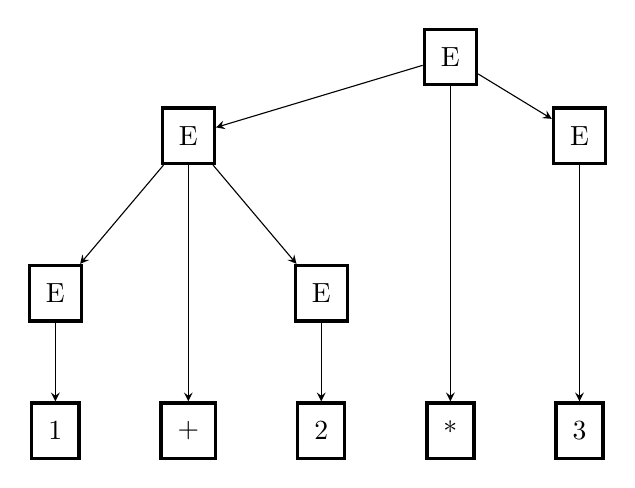
\begin{tikzpicture}[auto,
    ->,
  %  shorten >=2pt,
    >=stealth,
  %  node distance=1cm,
    bb/.style={%
      rectangle, draw=black, very thick, fill=white,
      text ragged, minimum height=2em, inner sep=6pt, align=center
    },
    inv/.style={%
      rectangle, draw=none, fill=white,
      text ragged, minimum height=2em, inner sep=6pt, align=center
    }
]
    \node[bb] (1)                  {1};
    \node[bb] (2)  [right = of 1]  {+};
    \node[bb] (3)  [right = of 2]  {2};
    \node[bb] (4)  [right = of 3]  {*};
    \node[bb] (5)  [right = of 4]  {3};
    \node[bb] (6)  [above = of 1]  {E};
    \node[bb] (7)  [above = of 3]  {E};
    \node[bb] (8)  [above = of 2, yshift = 2cm]  {E};
    \node[bb] (9)  [above = of 5, yshift = 2cm]  {E};
    \node[bb] (10) [above = of 4, yshift = 3cm]  {E};

    \path (6)  edge node {}  (1)
		  (7) edge node {}  (3)
		  (10) edge node {}  (4)
		  (10) edge node {}  (8)
		  (10) edge node {}  (9)
		  (9) edge node {}  (5)
		  (8) edge node {}  (7)
		  (8) edge node {}  (6)
          (8) edge node {}  (2)
    ;

  \end{tikzpicture}
}
\\
\pause
\checkmark & $\times$ \\

\end{tabular}

\end{center}
\end{scriptsize}
\end{frame}
% frame end %%%%%%%%%%%%%%%%%%%%%%%%


% frame begin %%%%%%%%%%%%%%%%%%%%%%%%
\begin{frame}[fragile]{Parsing}
{Handling Ambiguity -- Associativity}

\begin{scriptsize}
\begin{center}

\begin{tabular}{c @{\hspace{0.5cm}} c}
4 - 2 - 1
&
\begin{minipage}{0.5\textwidth}
\begin{tcolorbox}
\begin{tabular}{l @{} c @{} l}
$E$     & {\myprod}   & $E$ + $E$         \\
$E$     & {\myprod}   & $E$ - $E$         \\
$E$     & {\myprod}   & ($E$)             \\
$E$     & {\myprod}   & 0 $|$ 1 ... $|$ 9 \\
\end{tabular}
\end{tcolorbox}
\end{minipage}
\end{tabular}

\pause

- is left associative.
\end{center}

\pause


\begin{center}
\begin{tabular}{c @{\hspace{0.5cm}} c}
\resizebox{!}{0.35\textheight}{%
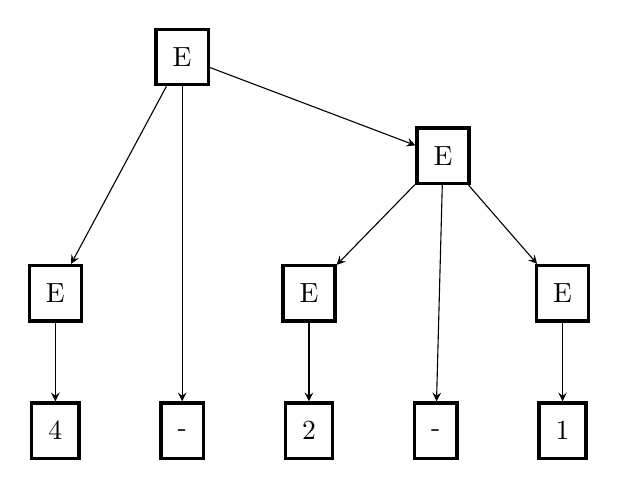
\begin{tikzpicture}[auto,
    ->,
  %  shorten >=2pt,
    >=stealth,
  %  node distance=1cm,
    bb/.style={%
      rectangle, draw=black, very thick, fill=white,
      text ragged, minimum height=2em, inner sep=6pt, align=center
    },
    inv/.style={%
      rectangle, draw=none, fill=white,
      text ragged, minimum height=2em, inner sep=6pt, align=center
    }
]
    \node[bb] (1)                  {4};
    \node[bb] (2)  [right = of 1]  {-};
    \node[bb] (3)  [right = of 2]  {2};
    \node[bb] (4)  [right = of 3]  {-};
    \node[bb] (5)  [right = of 4]  {1};
    \node[bb] (6)  [above = of 1]  {E};
    \node[bb] (7)  [above = of 3]  {E};
    \node[bb] (8)  [above = of 5]  {E};
    \node[bb] (9) [above right = of 7]  {E};
    \node[bb] (10) [above = of 2, yshift = 3cm]  {E};

    \path (6)  edge node {}  (1)
          (10) edge node {}  (2)
		  (10) edge node {}  (6)
		  (10) edge node {}  (9)
		  (9) edge node {}  (8)
		  (9) edge node {}  (4)
		  (9) edge node {}  (7)
		  (7) edge node {}  (3)
		  (8) edge node {}  (5)
    ;

  \end{tikzpicture}
}

&
\resizebox{!}{0.35\textheight}{%
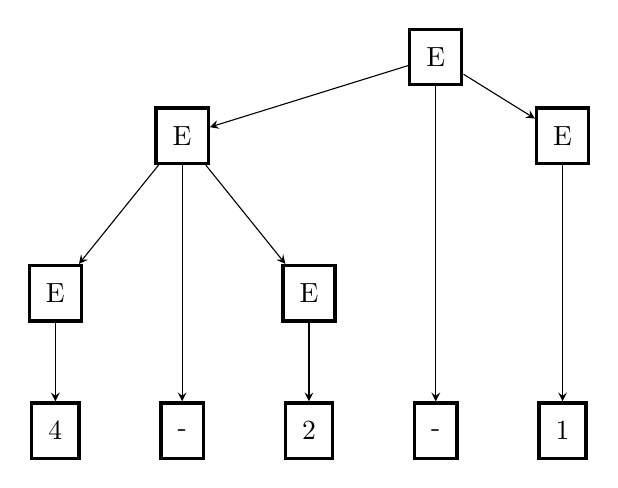
\begin{tikzpicture}[auto,
    ->,
  %  shorten >=2pt,
    >=stealth,
  %  node distance=1cm,
    bb/.style={%
      rectangle, draw=black, very thick, fill=white,
      text ragged, minimum height=2em, inner sep=6pt, align=center
    },
    inv/.style={%
      rectangle, draw=none, fill=white,
      text ragged, minimum height=2em, inner sep=6pt, align=center
    }
]
    \node[bb] (1)                  {4};
    \node[bb] (2)  [right = of 1]  {-};
    \node[bb] (3)  [right = of 2]  {2};
    \node[bb] (4)  [right = of 3]  {-};
    \node[bb] (5)  [right = of 4]  {1};
    \node[bb] (6)  [above = of 1]  {E};
    \node[bb] (7)  [above = of 3]  {E};
    \node[bb] (8)  [above = of 2, yshift = 2cm]  {E};
    \node[bb] (9)  [above = of 5, yshift = 2cm]  {E};
    \node[bb] (10) [above = of 4, yshift = 3cm]  {E};

    \path (6)  edge node {}  (1)
		  (7) edge node {}  (3)
		  (10) edge node {}  (4)
		  (10) edge node {}  (8)
		  (10) edge node {}  (9)
		  (9) edge node {}  (5)
		  (8) edge node {}  (7)
		  (8) edge node {}  (6)
          (8) edge node {}  (2)
    ;

  \end{tikzpicture}
}
\\
\pause
$\times$ & $\checkmark$ \\

\end{tabular}

\end{center}
\end{scriptsize}
\end{frame}
% frame end %%%%%%%%%%%%%%%%%%%%%%%%

% frame begin %%%%%%%%%%%%%%%%%%%%%%%%
\begin{frame}{Parsing}
{Ambiguity}

\begin{itemize}
\item Language processors can't deal with ambiguity.
\item Ambiguous grammars are common.
\item Methods of dealing with ambiguity:
\begin{itemize}
	\item Fixing the grammar
	\item Associativity
	\item Operator precedence
\end{itemize}
\item Non-trivial
\item Not covered
\end{itemize}
\pause

\begin{center}

\begin{tikzpicture}
\node[rectangle, draw=Red, fill=Red]{};
\end{tikzpicture}
\end{center}
\end{frame}

% frame end %%%%%%%%%%%%%%%%%%%%%%%%


% frame begin %%%%%%%%%%%%%%%%%%%%%%%%
\begin{frame}{Next}

\myheader{Recursive Descent Parsing}
\end{frame}
% frame end %%%%%%%%%%%%%%%%%%%%%%%%

\end{document}
